\section{Ingeniería de detalle}\label{sec:ingdetalle}

% Es el conjunto de documentación técnica completa del proyecto que
% permite que la ejecución de éste sea entregada a un tercero y éste
% pueda efectuar la Instalación y Puesta en Marcha con mínimas
% variaciones.

% La Instalación y Puesta en marcha de un proyecto no necesariamente
% debe ser ejecutada por el grupo de trabajo que prepara la Ingeniería
% de Detalle. El ejecutor puede ser otra sección dentro de la misma
% Empresa o una Empresa contratista (Outsourcing). Por este motivo la
% Ingeniería de detalle debe ser completa y muy precisa. No deben quedar
% detalles sin definir.

% Dentro de la Ingeniería de detalle de un proyecto, y dependiendo de la
% naturaleza de éste, se pueden incluir los siguientes elementos:

% Planos de planta de las estaciones, especificando ubicación y
% dimensiones de los racks que alojarán a los equipos nuevos Layout de
% los equipos, esto es, planos frontales de los racks indicando la
% disposición de los equipos.

% Diagramas en bloque de los equipos indicando las interconexiones de
% los diferentes módulos (no se trata de los diagramas de circuitos
% electrónicos de cada tarjeta, información que los fabricantes no
% suelen entregar, sino que de las conexiones externas entre las
% diferentes tarjetas, para conseguir que los equipos trabajen en la
% forma deseada).

% Diagrama de cross-conexiones entre las diferentes interfaces de línea
% y las puertas tributarias de los equipos.  Plan de sincronización de
% la Red Planos de Planta Externa Memorias de cálculo
 
 
% El último elemento requiere de explicaciones adicionales.
 
% Una Memoria de Cálculo, como su nombre indica, es el resultado de los
% análisis y cálculos que efectúa un ingeniero especialista en una
% materia para determinar la forma correcta como debe ejecutarse una
% parte del proyecto para que el sistema funcione correctamente y de
% acuerdo a lo esperado.
 
% La memoria de cálculo puede ser de varios tipos según el
% proyecto. Algunos ejemplos:
 
% Memoria de cálculo de malla de tierra. Arroja como resultado
% especificaciones sobre la geometría de la malla, profundidad y número
% de las barras de cobre que deben enterrarse, valor de resistividad del
% terreno al cual debe llegarse.
 
% Memoria de cálculo de un radio enlace. Incluye un perfil del enlace,
% cálculos de niveles de señal, atenuaciones de las guías de onda y
% filtros, ganancia de las antenas, potencias de salida de los
% transmisores y nivel de recepción. Pero lo más importante es el
% cálculo de predicción de comportamiento del enlace en el peor mes del
% año, esto es \% del tiempo que el enlace estará indisponible (Tasa de
% error peor que 1E-03) y \% del tiempo que el enlace estará degradado
% (Tasa de error peor que 1E-06). Todos los métodos de cálculo y valores
% límites para los porcentajes mencionados están detallados por el ITU.
 
% Memoria de cálculo de enlaces por fibra óptica. Este tema es de
% importancia para el proyecto que les corresponde desarrollar. estos
% cálculos incluyen: balance de potencia; cálculo de razón señal a ruido
% óptica (OSNR) y cálculos de dispersión.
 
% Los resultados de estos cálculos determinan el diseño de la red y por
% lo tanto tiene impacto en el CAPEX y OPEX del proyecto: tipo de
% interfaces ópticas (estándar, de alta potencia, Ultra alta potencia),
% necesidad de usar Amplificadores Ópticos de Línea (OLA) o
% Regeneradores intermedios en un enlace.
 
% El impacto en el CAPEX es claro, si el diseño arroja que es necesario
% incluir una estación regeneradora en medio de un enlace entre
% estaciones ya existentes, el costo del proyecto se eleva notablemente.
 
% Por otra parte, un diseño muy audaz puede significar una reducción del
% margen disponible en el enlace, lo cual ante una degradación menor del
% cable de fibra puede hacer que el enlace se corte o degrade, obligando
% a efectuar mantenimiento con más frecuencia y elevando el OPEX.
 
% Memoria de cálculo de una torre. En un proyecto que incluya enlaces de
% microondas y emplazamiento de radio estaciones nuevas con sus
% receptivas torres, se debe incluir el cálculo de la estructura de la
% torre para asegurar su resistencia al peso de las antenas, al viento,
% etc. Naturalmente este cálculo cae dentro de las responsabilidades de
% un Ingeniero Civil no Eléctrico.

En esta sección se presentará la ingeniería de detalle para el
proyecto de implementación de red óptica utilizando \emph{DWDM} y
\emph{ROADM} con \emph{WSS} basado en un enfoque probabilístico para
diseño de caminos óptimos a partir de valores esperados del
\emph{SLA}.

La ingeniería de detalle expuesta aquí es una recopilación de todos
los documentos técnicos que se requieren para la instalación física de
los equipos y la programación de los \emph{ROADM}. Esta recopilación
se basa en el diseño final seleccionado de entre las propuestas de los
proveedores en la sección \ref{sec:ppfinal}.

\subsection{Diagramas de conexión ROADM}
\label{sec:diagramasroadm}

El detalle de las conexiones de equipos en cada uno de los \emph{DC}
se presenta en las siguientes secciones.

\subsubsection{Conexión ROADM ``Ciudad de los valles''}
\label{sec:drcdv}

\begin{figure}[H]
  \centering
  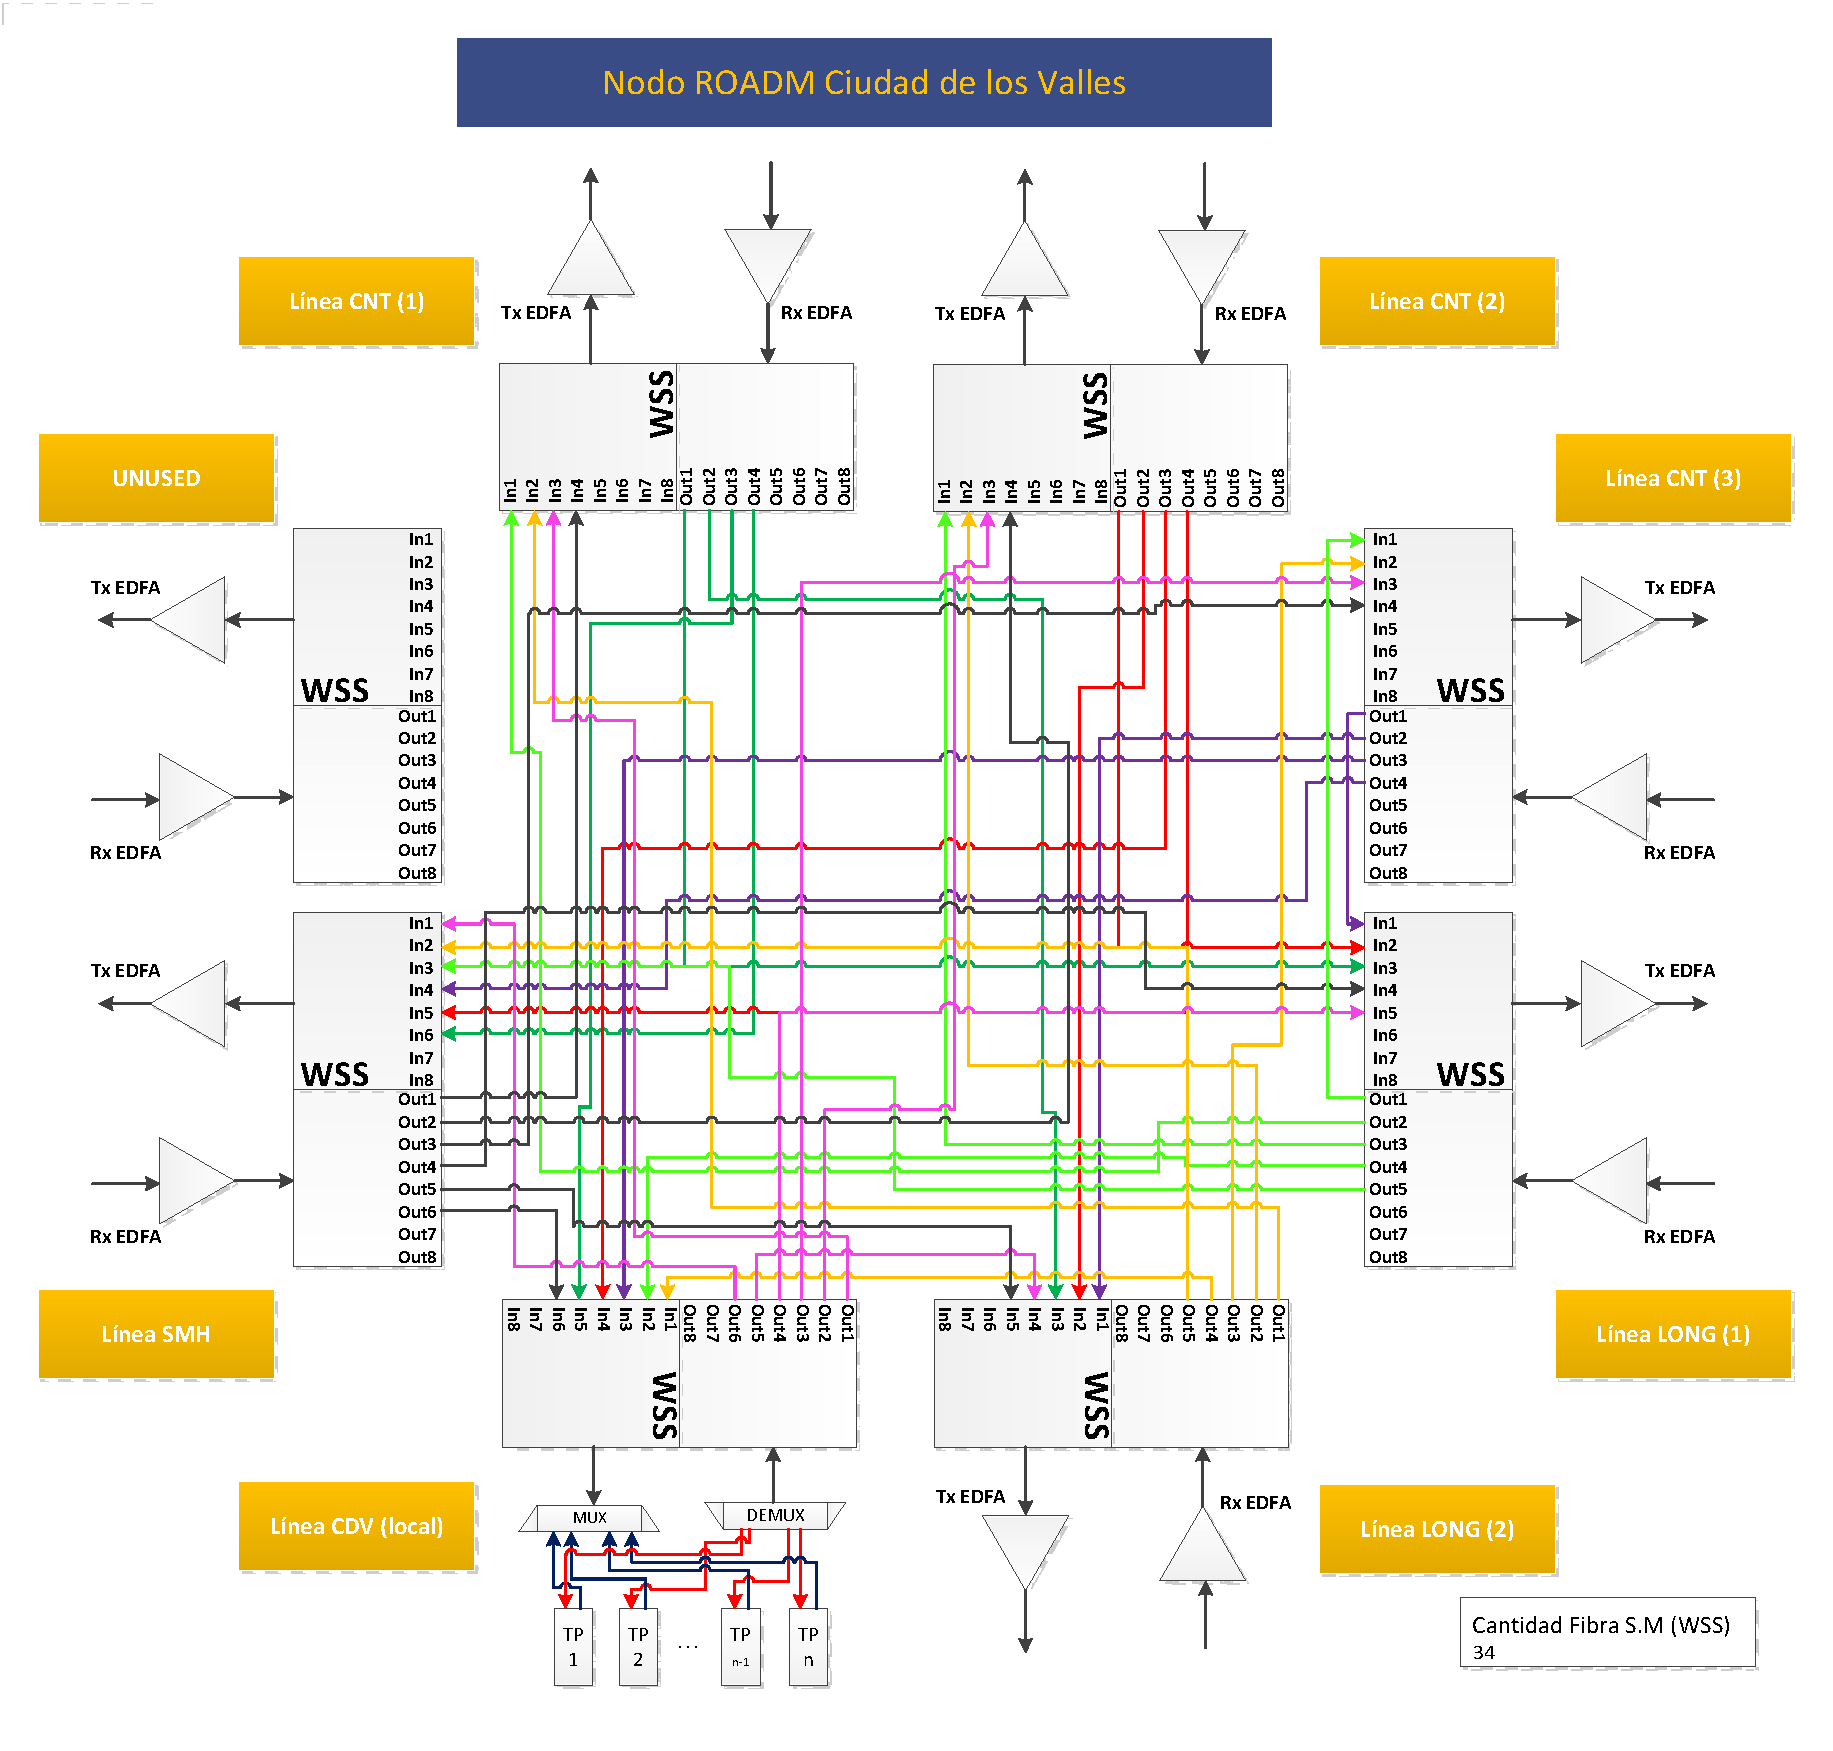
\includegraphics[width=17cm]{Imagenes/CDV.pdf}
  \caption{Diagrama de conexión de equipos para infrastructura ROADM
    en ``Ciudad de los valles''}
  \label{fig:drcdv}
\end{figure}

\subsubsection{Conexión ROADM ``Central nacional de
  telecomunicaciones''}
\label{sec:drcnt}

\begin{figure}[H]
  \centering
  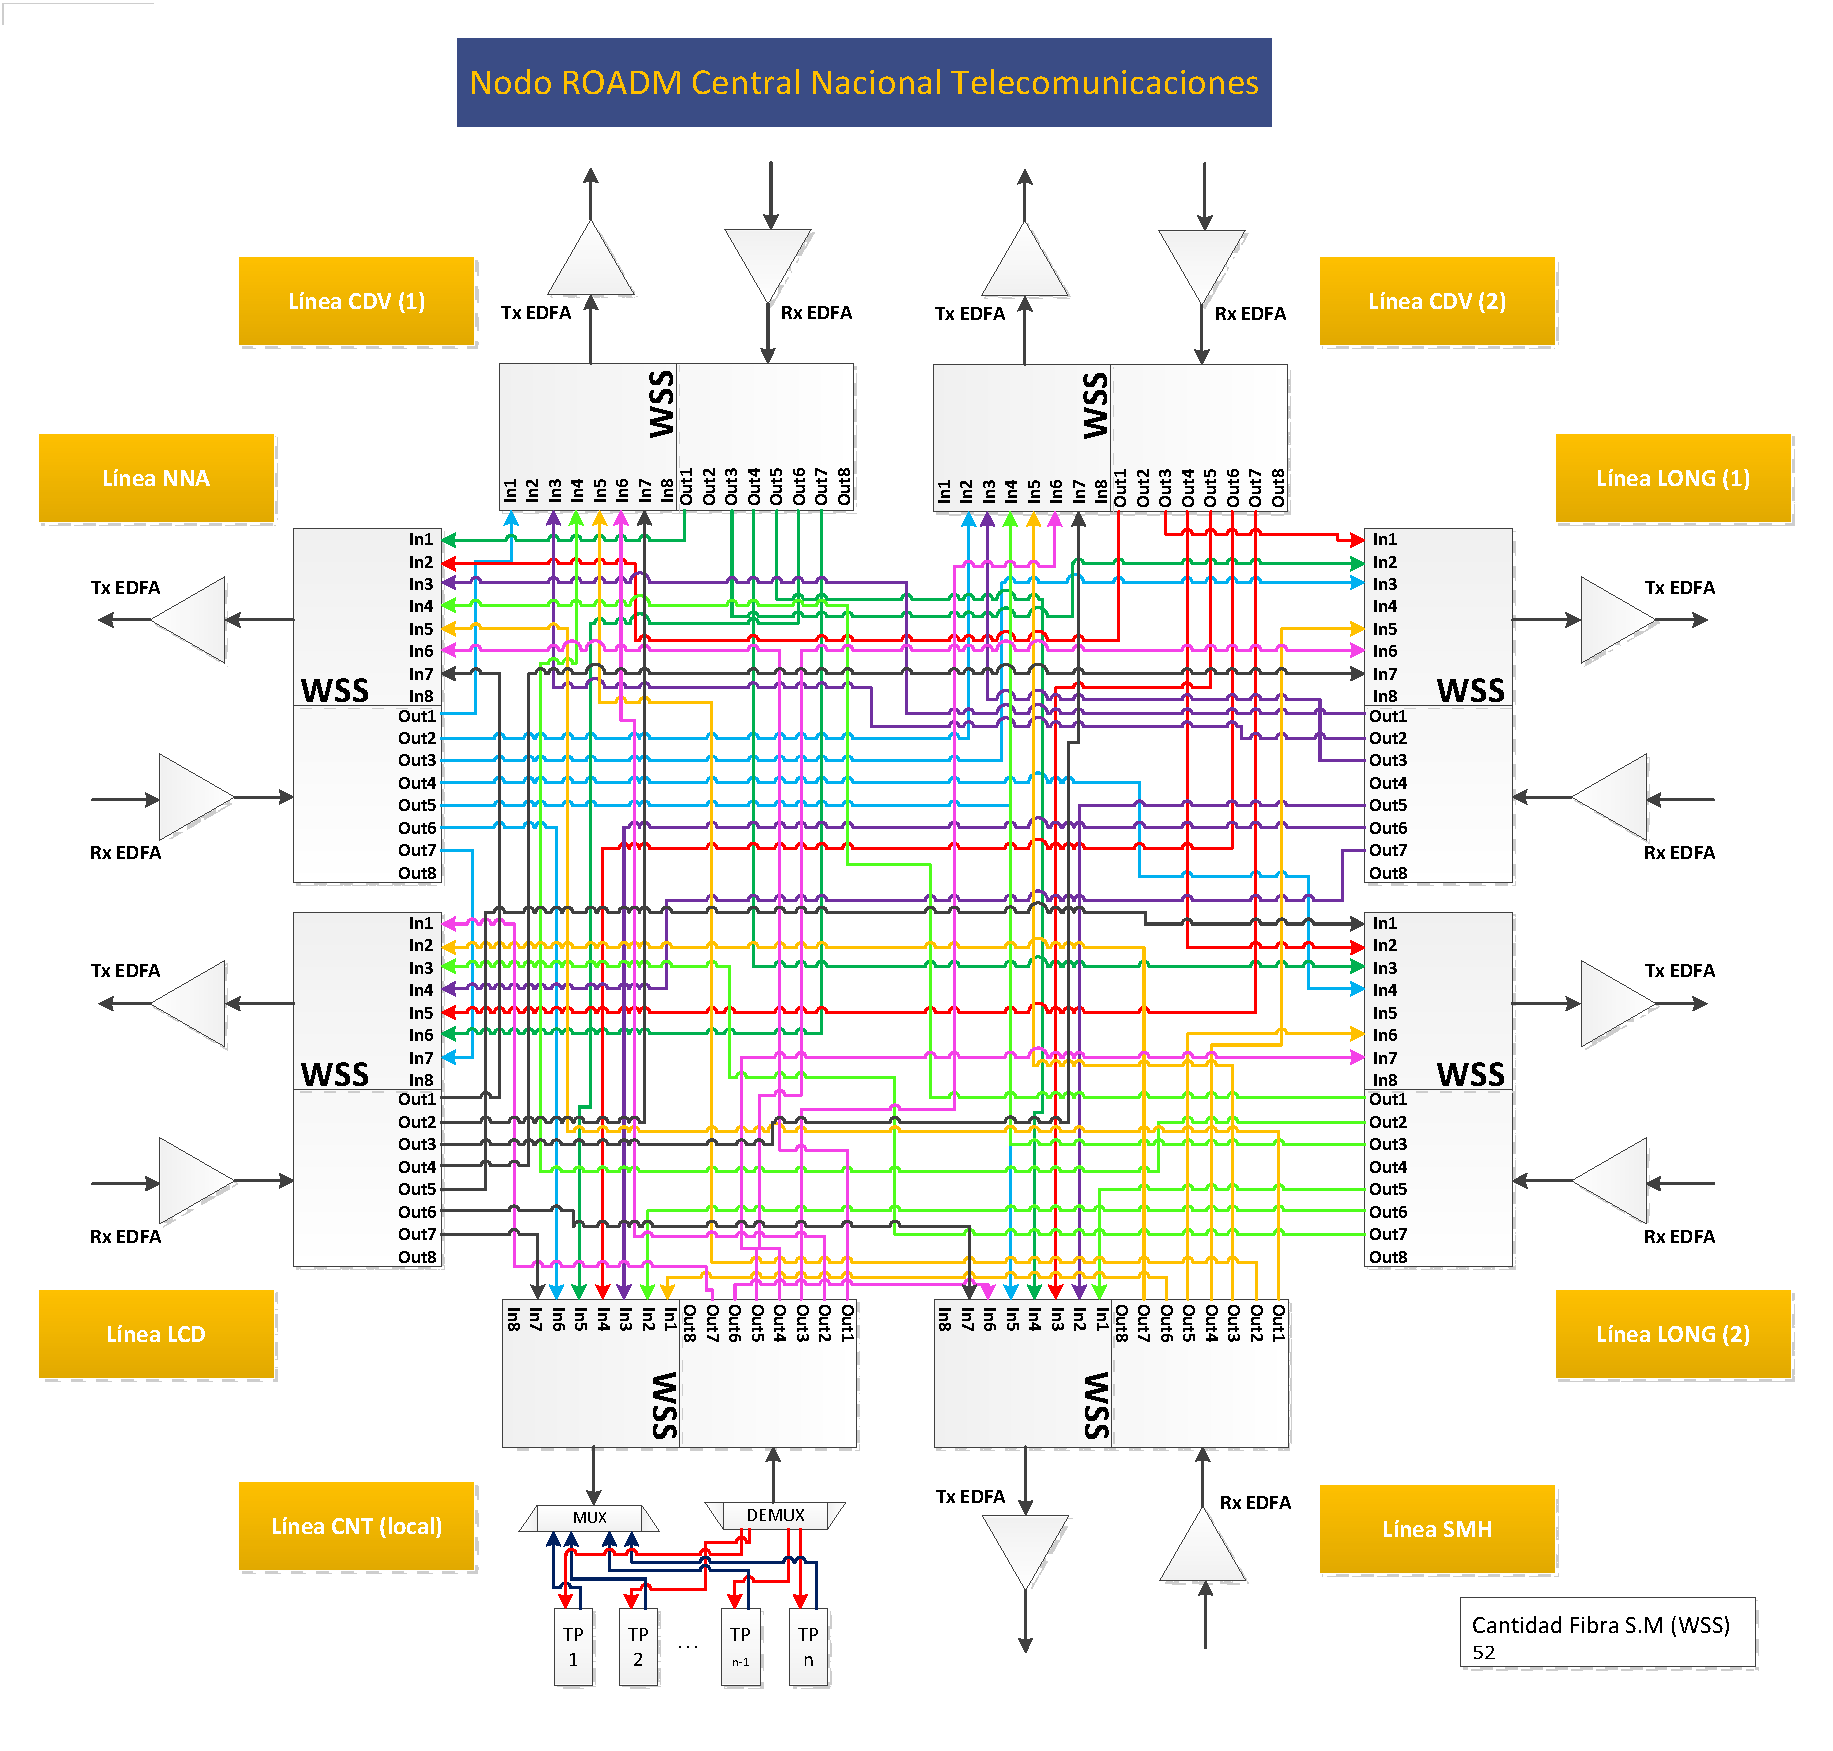
\includegraphics[width=17cm]{Imagenes/CNT.pdf}
  \caption{Diagrama de conexión de equipos para infrastructura ROADM
    en ``Central nacional de telecomunicaciones''}
  \label{fig:drcnt}
\end{figure}

\subsubsection{Conexión ROADM ``Las Condes''}
\label{sec:drlcd}

\begin{figure}[H]
  \centering
  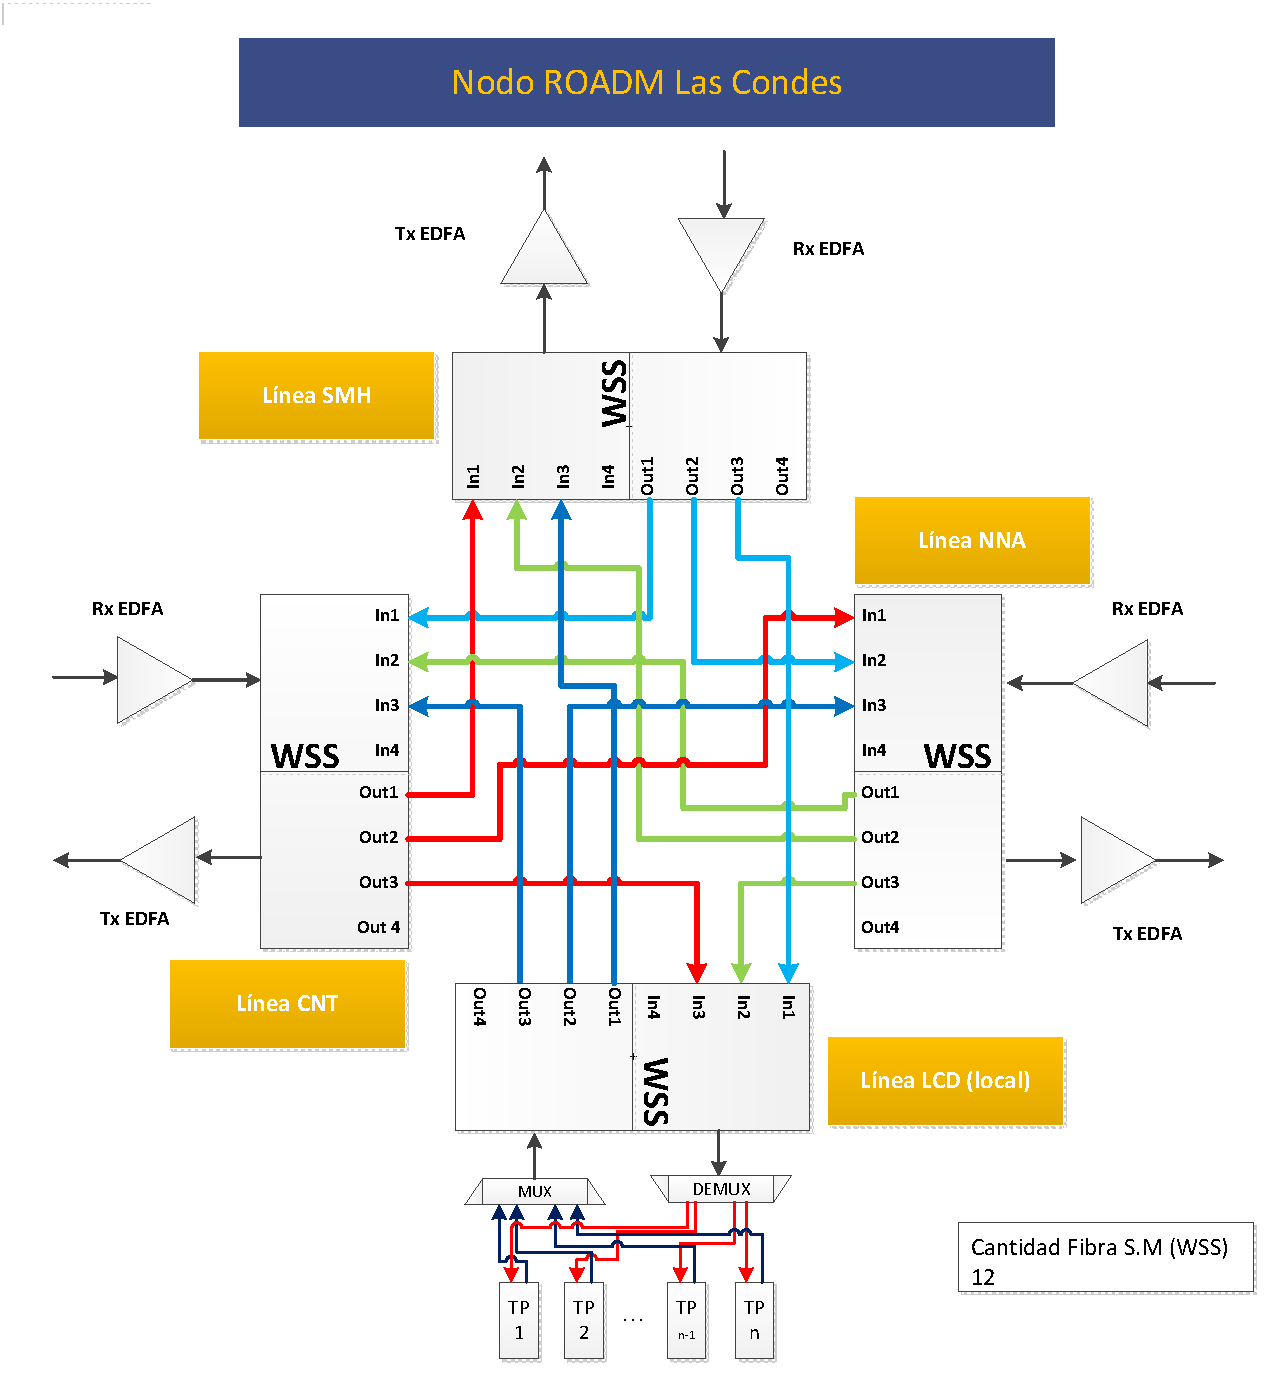
\includegraphics[width=17cm]{Imagenes/LCD.pdf}
  \caption{Diagrama de conexión de equipos para infrastructura ROADM
    en ``Las Condes''}
  \label{fig:drlcd}
\end{figure}

\subsubsection{Conexión ROADM ``Longovilo''}
\label{sec:drlong}

\begin{figure}[H]
  \centering
  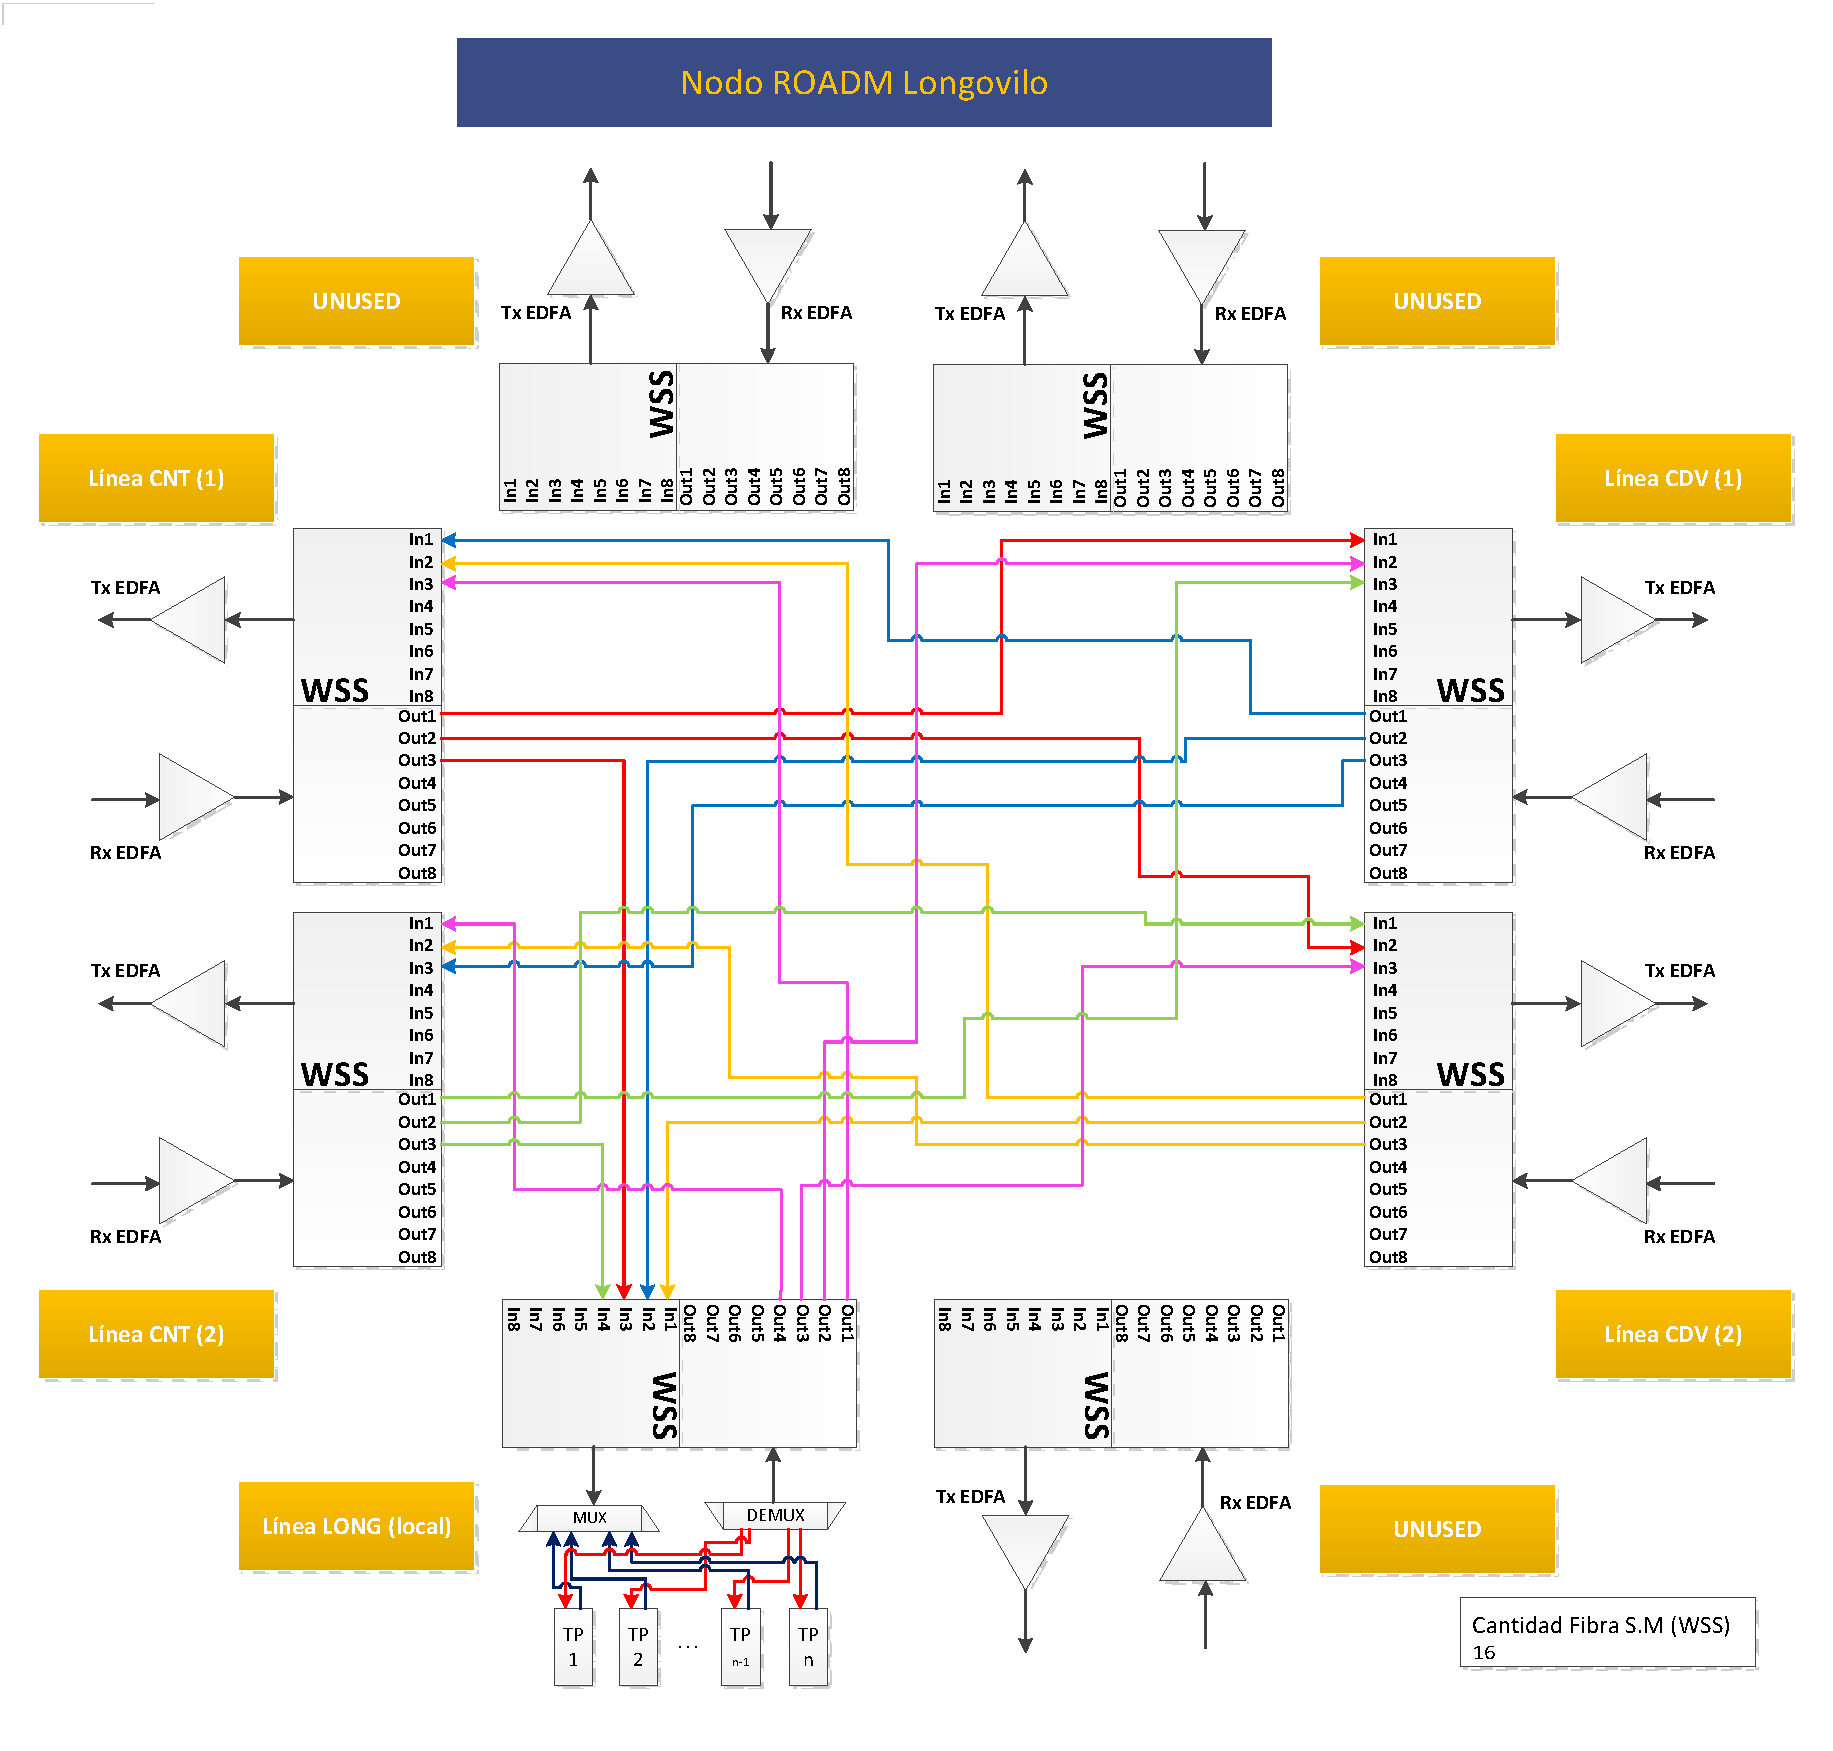
\includegraphics[width=17cm]{Imagenes/LONG.pdf}
  \caption{Diagrama de conexión de equipos para infrastructura ROADM en ``Longovilo''}
  \label{fig:drlong}
\end{figure}

\subsubsection{Conexión ROADM ``Ñuñoa''}
\label{sec:drnna}

\begin{figure}[H]
  \centering
  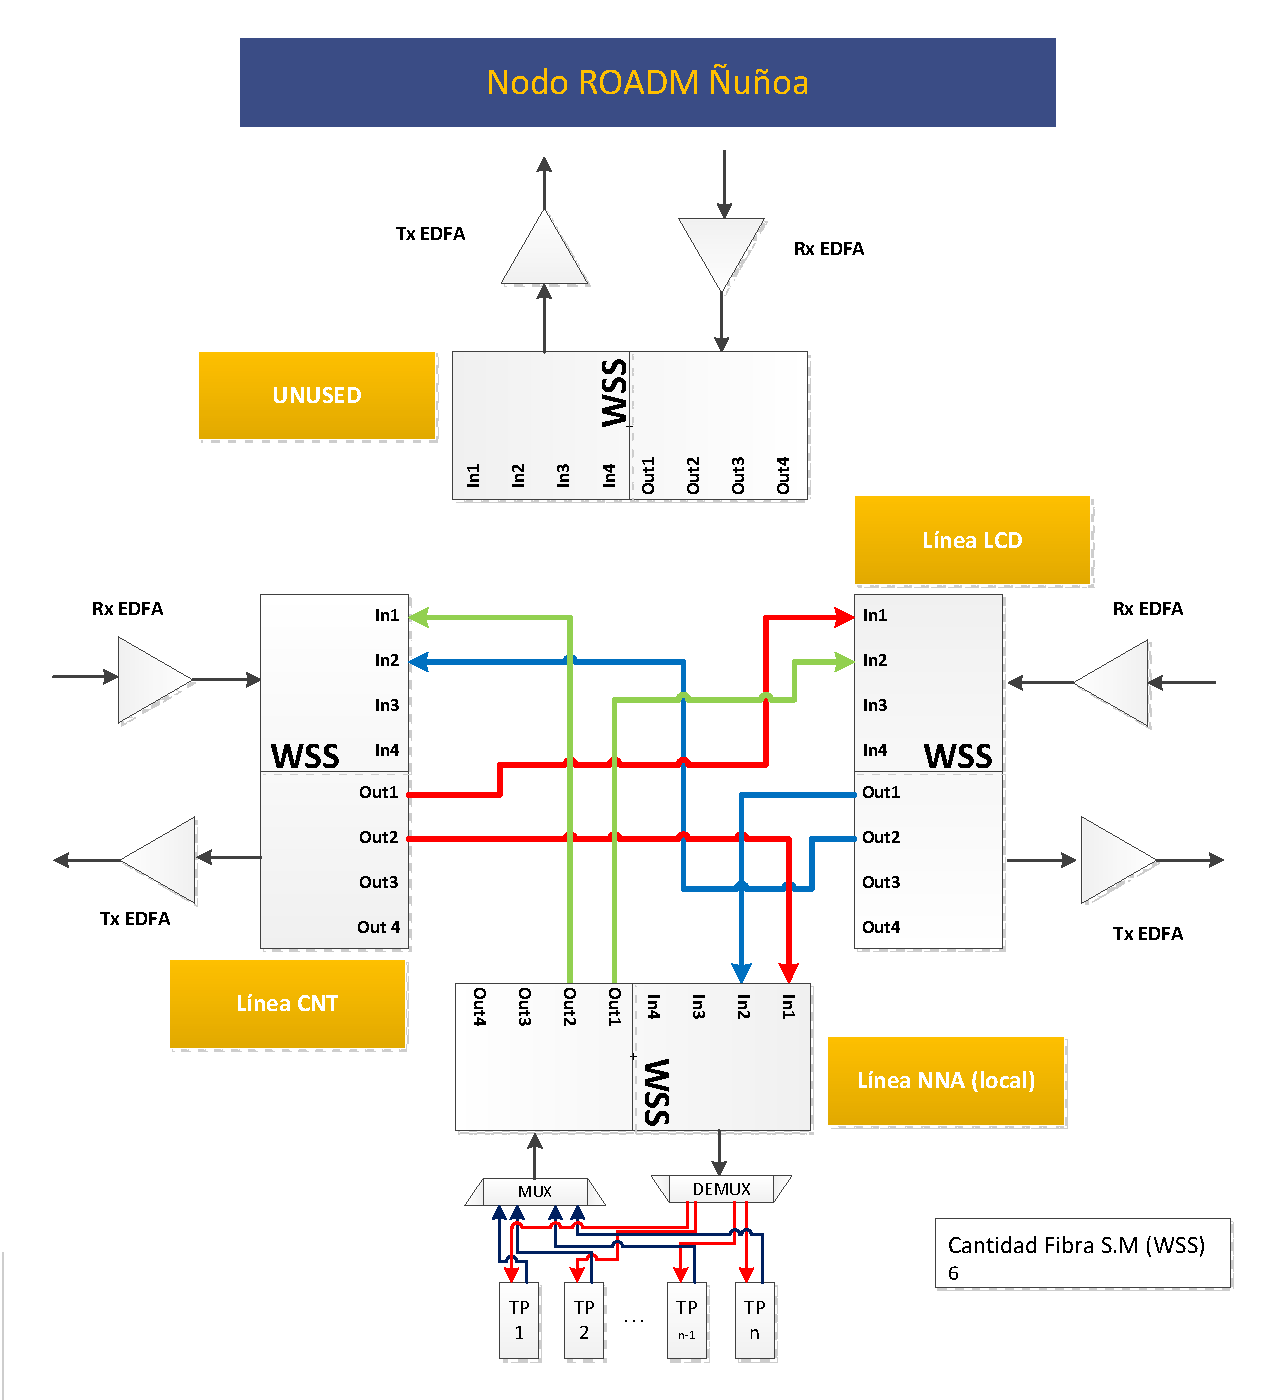
\includegraphics[width=17cm]{Imagenes/NNA.pdf}
  \caption{Diagrama de conexión de equipos para infrastructura ROADM en ``Ñuñoa''}
  \label{fig:drnna}
\end{figure}

\subsubsection{Conexión ROADM ``Santa Marta de Huechuraba''}
\label{sec:drsmh}

\begin{figure}[H]
  \centering
  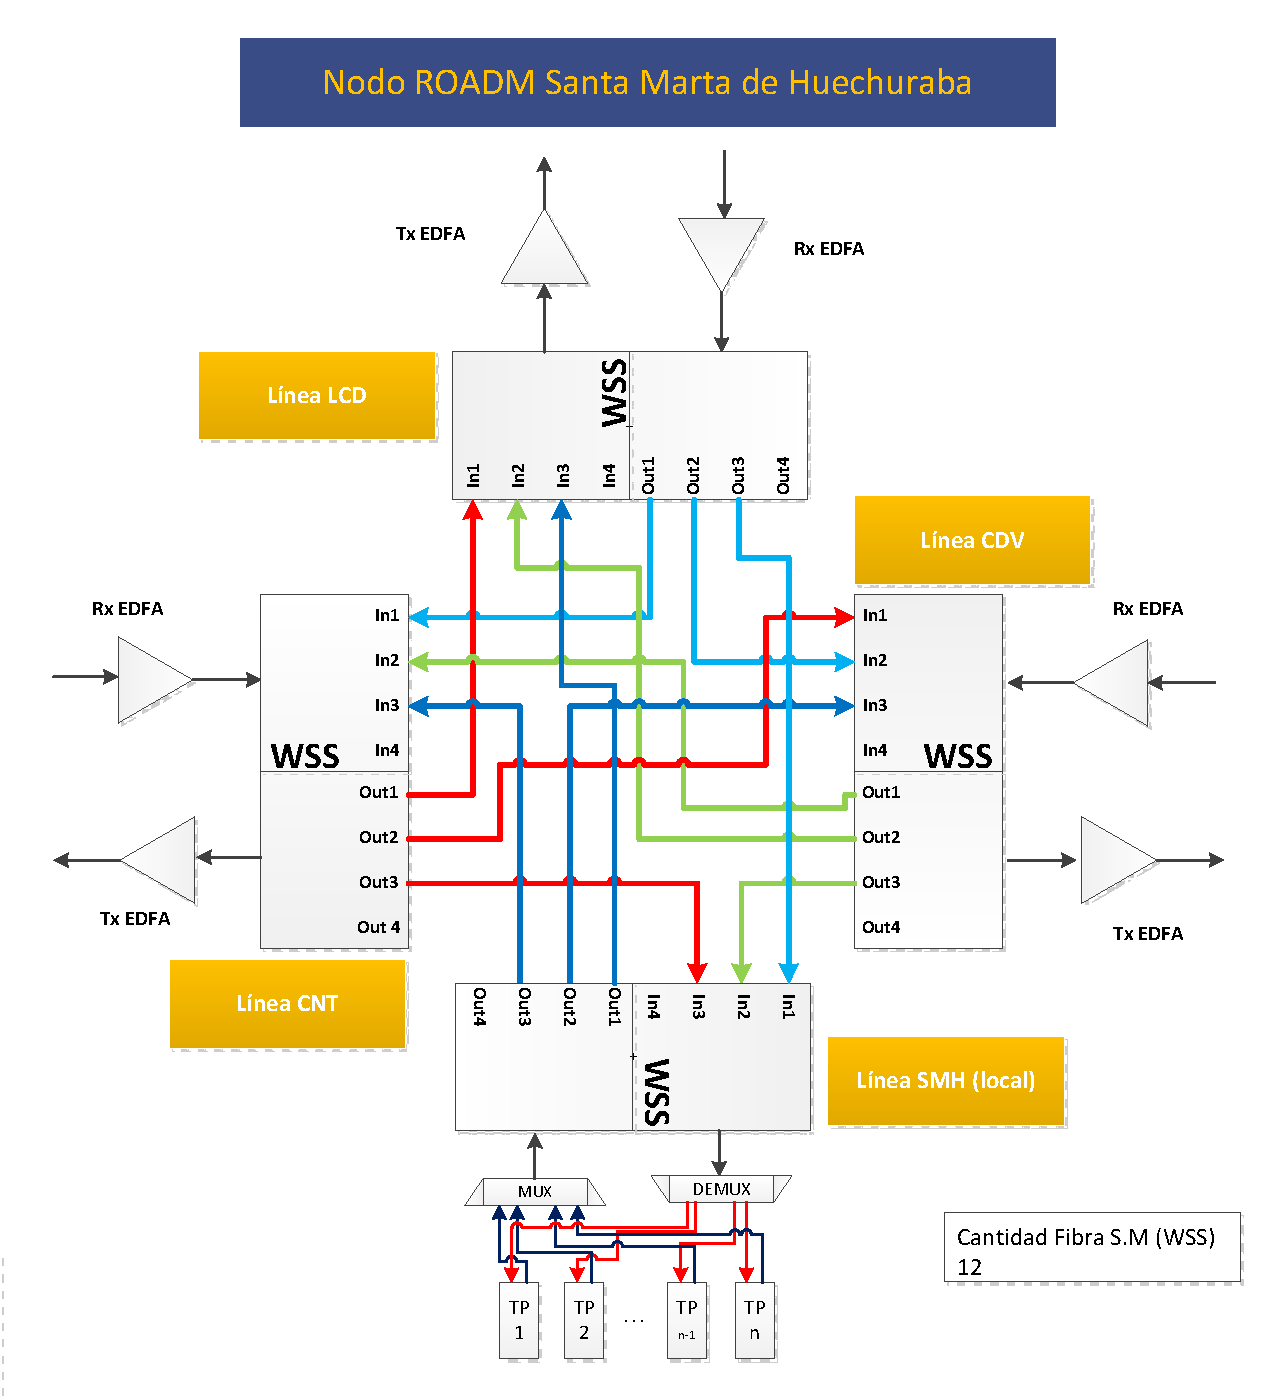
\includegraphics[width=17cm]{Imagenes/SMH.pdf}
  \caption{Diagrama de conexión de equipos para infrastructura ROADM en ``Santa Marta de Huechuraba''}
  \label{fig:drsmh}
\end{figure}

\subsection{Montaje de racks}
\label{sec:racks}

Los racks utilizados en cada \emph{DC} se instalan de la misma manera,
tal y como se muestra en el diagrama \ref{fig:racks}.

\begin{figure}[H]
  \centering
  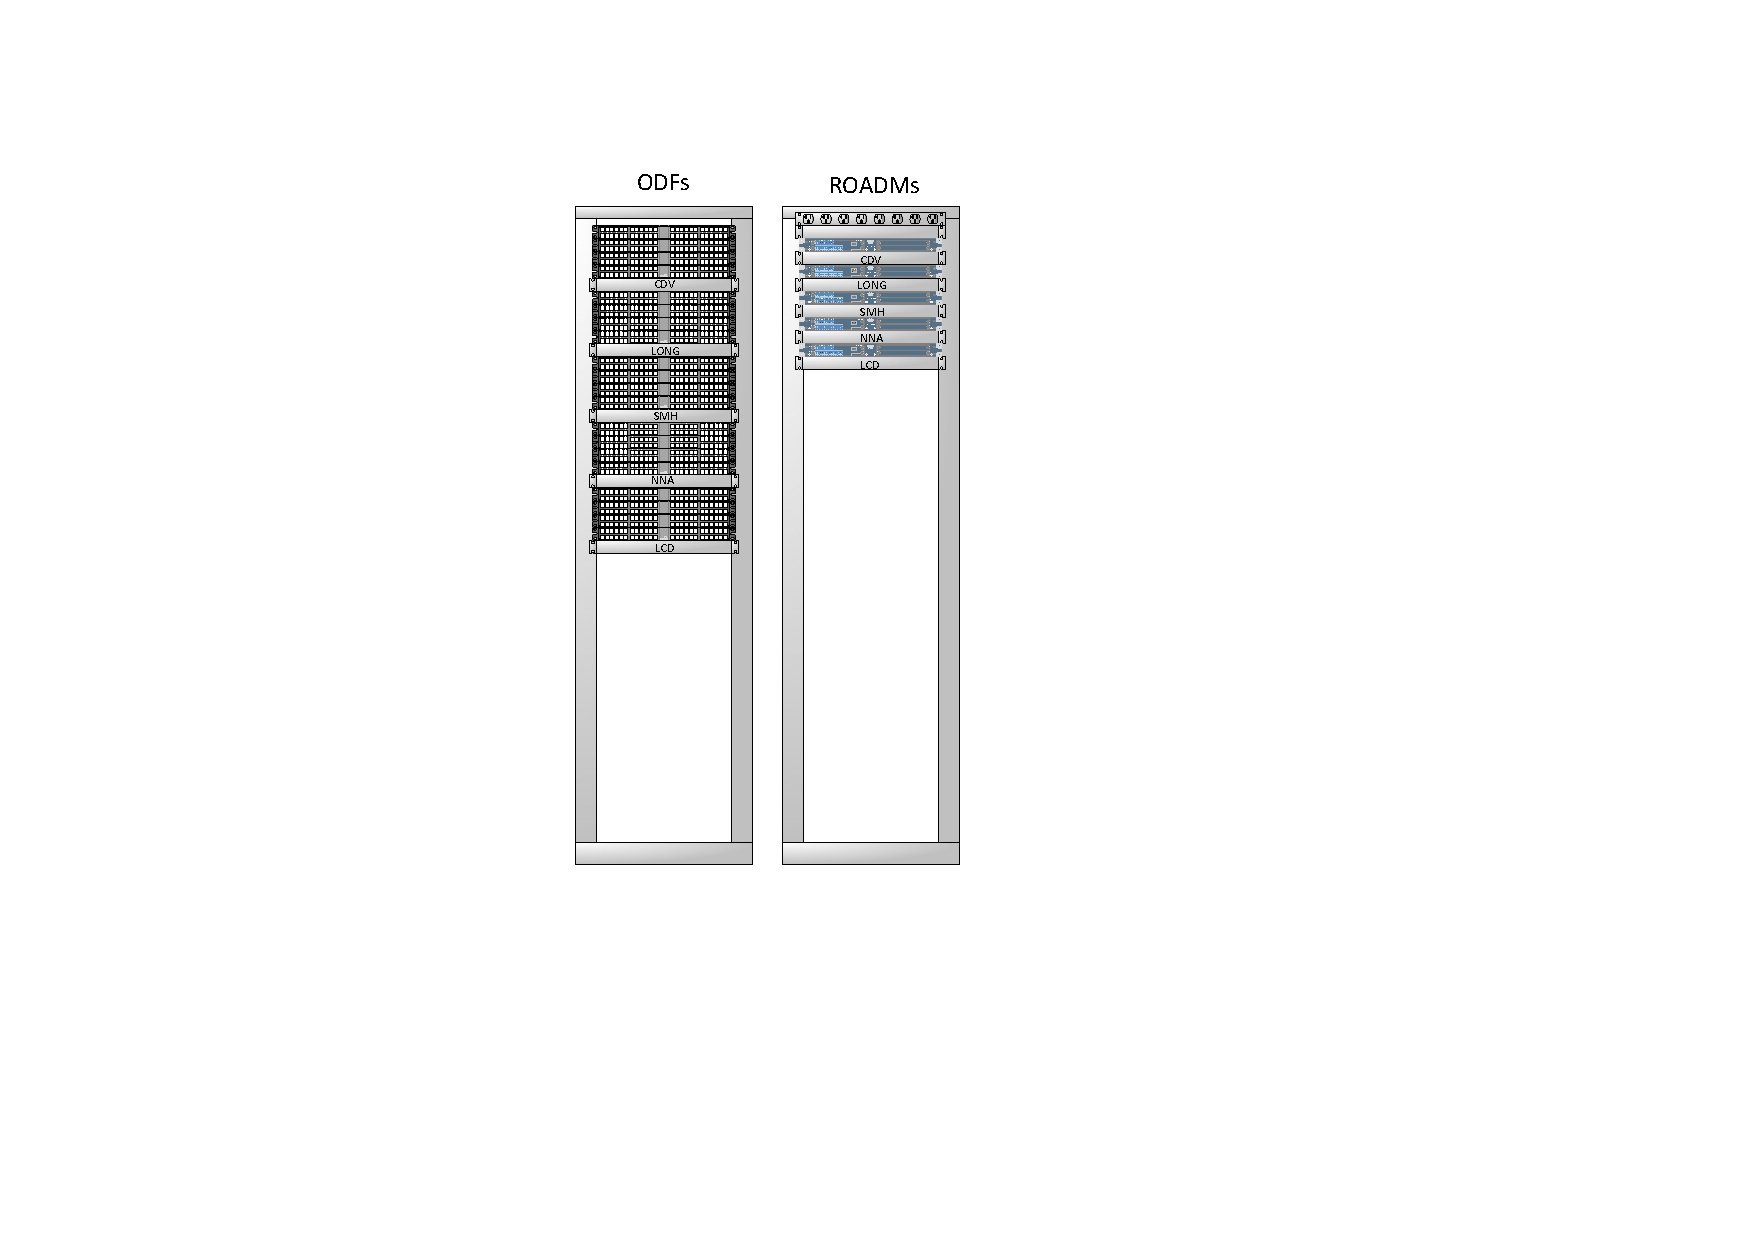
\includegraphics[width=12cm]{Imagenes/racks3.pdf}
  \caption{Montaje de racks en los data centers}
  \label{fig:racks}
\end{figure}

Cada \emph{DC} deberá contar con un rack para albergar y proteger los
ODF (puntos de red de la fibra óptica) y uno para almacenar los
equipos \emph{ROADM}.

El rack de \emph{ROADM}, a su vez, debe seguir las conexiones
mostradas en la sección \ref{sec:diagramasroadm}.

\subsection{Anexo: cálculo OSNR}
\label{sec:osnr}

El \emph{OSNR} (\emph{optical signal to noise ratio}) es el cuociente
entre la intensidad de la señal y la intensidad del ruido en redes
ópticas. Se calcula al final de la línea compuesta por \emph{EDFA}'s
(\emph{erbium doped fiber amplifiers}) en distintos puntos del enlace
y por fibra que los une. Esta última actúa como atenuador. Los
amplificadores generan ruido.

Para calcular el OSNR se debe calcular la potencia de recepción y la
intensidad del ruido, y luego calcular su cuociente. Es conveniente
usar los decibeles como unidades ya que para calcular el cuociente
basta con calcular la diferencia entre ambos resaltados.

La potencia final del enlace (potencia en el receptor) es igual
a $$P_f=P_0\frac{g_Bg_{PA}}{L}$$ donde $P_0$ es la potencia de
entrada, $g_b$ es la ganancia del booster en $mW$, $g_{PA}$ es la
ganancia del preamplificador en $mW$ y $L$ es la atenuación de la
fibra.

El ruido que inyecta un amplificador se puede calcular usando la
fórmula: $$n = fgn_0$$ $f$ es el valor de ruido que inyecta el
amplificador, $g$ es la ganancia de ese amplificador y $n_0$ es una
constante para \emph{DWDM} igual a $-58 dB$. $f$ y $g$ están en $mW$
en esa fórmula, aunque los fabricantes entregan el valor en decibeles
(requiere transformación).

Es necesario considerar que los amplificadores tienen una salida
máxima que no puede sobrepasarse. Esto se tomó en cuenta en los
cálculos realizados a continuación.

Los parámetros en este caso son los que se muestran en la tabla
\ref{tab:parametros}.

\begin{table}[H]
  \centering
  \begin{tabular}{| c | r | r |}
    \hline
    Parámetros & Valores en dB & Valores en mW relativos \\
    \hline
    Entrada & $0$ & $1$ \\
    G & $22$ & $158,5$ \\
    F & $6$ & $3,981$ \\
    $h \nu \Delta \nu$ & $-58$ & $1,585E-06$ \\
    Att FO & $0,24$ & $1,057$ \\
    $P_{outMax}$ & $18$ & $63,10$ \\
    \hline
  \end{tabular}
  \caption{Tabla de parámetros}
  \label{tab:parametros}
\end{table}

Los cálculos de la tabla \ref{tab:osnr1} muestran los resultados de
intensidad de la potencia de la señal al final de cada enlace para
la red propuesta.

\begin{table}[H]
  \centering
  \begin{tabular}{| l | c | c | c | c | c |}
    \hline{}
    Enlace & Distancia (Km.) & Atenuación (dB) & $P_{out}$ (dB) & Ruido (dB) & OSNR (dB) \\

    \hline
    CDV-SMH  & 30  & 7,2   & 18   & -15,06 & 33,06 \\
    CDV-LONG & 110 & 26,4  & 13,6 & -28,65 & 42,25 \\
    CDV-CNT  & 45  & 10,8  & 18   & -18,48 & 36,48 \\
    SMH-CNT  & 20  & 4,8   & 18   & -12,72 & 30,72 \\
    SMH-LCD  & 25  & 6     & 18   & -13,89 & 31,89 \\
    CNT-LCD  & 12  & 2,88  & 18   & -10,83 & 28,35 \\
    CNT-NNA  & 10  & 2,4   & 18   & -10,35 & 28,35 \\
    NNA-LCD  & 15  & 3,6   & 18   & -11,54 & 29,54 \\
    LONG-CNT & 132 & 31,68 & 8,32 & -29,56 & 37,88 \\
    \hline
  \end{tabular}
  \caption{Tabla de cálculos de \emph{OSNR} por enlace.}
  \label{tab:osnr1}
\end{table}

El valor de \emph{OSNR} obtenido es satisfactorio para un diseño como
el propuesto, ya que el umbral supera los $18dB$ mínimos de un sistema
que utiliza tranpondedores no coherentes de 10 Gb, como es este el
caso. En efecto, si los valores son demasiado altos se pueden atenuar
utilizando para ello atenuadores.
